

This chapter is dedicated to the methodology that we propose to exert to achieve the objectives of this research project, i.e. Methodology and Algorithms for High-level Modeling of Cosmic Radiations Impacts on Electrical Systems.

\section{Relation to State-of-the-Art}
Starting from the background, the facts established in the Chapter~\ref{intro}--- the digital circuits vulnerable to radiations require high-reliability requirements. The faults due to particle strikes cause different effects in the system behavior, e.g., stuck-at-fault. As discussed in~\ref{related}.The previous work on soft error analysis and evaluation, the researchers are focused on the low abstractions level. Most of the work done based on the interaction of the cosmic rays with the silicon atoms and its analysis, prediction of error,  and estimating the model of transistors and circuit layout structure that can tolerate radiations effects. On circuit level researchers are more focused on the generation and propagation of the radiation-induced transient pulses. The effects of these pulses are simulated with the help of SPICE. These fundamental analysis is important and provide insight of soft error rate. However, they can not take the overall erroneous behavior of the circuit at the architecture level, the errors produced at the low level propagate to the high level of abstraction. Further, the increased complexity of integrated circuits, and integration of several components, it is more difficult now to do the low-level circuit analysis and make the model at low-level. It is more viable solution to find the faulty response of the circuit at low level and model it to the high-level of abstraction. The high-level design suppresses a lot of unnecessary details, reduce the complexity, and its closer to the designer way of thinking. Our problem is unique in terms that it involve emulation of the hardware and behavioral model, to find the faulty response of the system. As can be depicted from the Figure~\ref{fig:ychart}.

The objective of the thesis is to construct a model from the faulty response observed at low-level circuit fault emulation. This model provide the response of the system under fault. It can be described with Y-chart as shown in Figure~\ref{fig:ychart}, in which the high-level analysis (Behavioral View) based on the faulty response at the circuit level. In high-level abstractions level the detailed of the implemented design is hide from the designer, therefore the designer believe that the source of errors to occur is bit-upset. In this work, we propose a solution to solve the problem (mimic the low-level faulty response to the high-level behavioral model) based on the Hidden Markov Model, that uses the concept of hidden states and observed states to find not only the hidden states of the faulty system but also accurately predict the observed states. 


\begin{figure}[tb!]

 \centering
  \captionsetup{justification=centering}    
   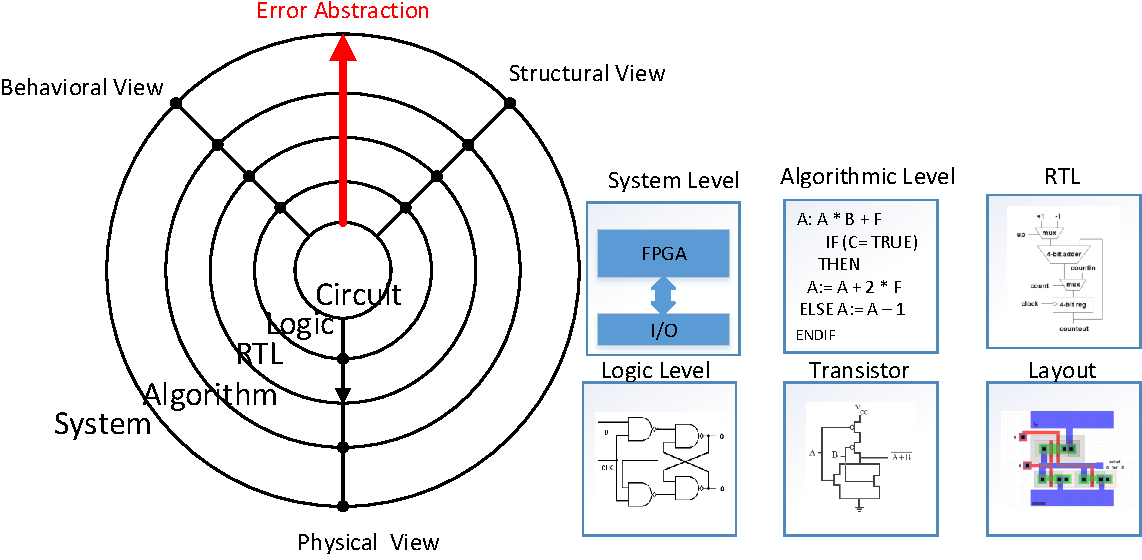
\includegraphics[scale=0.8]{Figures/ychart-block.pdf}
   \caption{Contribution of this work on Gajski-Kuhn chart.}
\label{fig:ychart}
\end{figure}

\section{Why Hidden Markov Model?}

The HMM is called hidden because only the outputs emitted by the system are observable (signatures --- in ours problem domian), not underlying states of the system (Stuck-at-fault). The HMM can be visualized as a simple finite state machine. The HMM has a strong statistical foundation; it has the ability for efficient learning algorithm, which can take place directly from the raw sequence data. \textbf{The problem in hand:} can be solved by using the HMM as we can observe the sequence of signatures, but we do not know the which states of the system went through to generate that particular signature. The analyses of Hidden Markov Model seek to recover the states from the observed data.



\section{Preliminaries of Hidden Markov Model}


Hidden Markov Model is a statistical model in which a system can be modeled is assumed to be a Markov process with unobserved, i.e., hidden states. 

\begin{tcolorbox}[width=\textwidth,colback={gray},title={Markov Process},colbacktitle=gray,coltitle=black]  

A Markov process  is a stochastic process that satisfies the Markov property -- \underline{memorylessness}, meaning, a process that satisfies the Markov property if the prediction of the future of the system output based solely on its present state, it is independent of the future and past states.   
\end{tcolorbox}


Inorder to apply the HMM, we need a system that generate probabilistic output patterns in time, e.g., faulty response of the 3-bit counter, as a result the node is stuck. Afterwards, we need to look at the system where we want to predict is not what we observe ---  the underlying system is hidden. For example, in the case of a three bit counter, the observed sequence is the "signature" and the hidden is the "stuck-at-node." Now, we wish to devise an algorithm to predict "stuck-at-node", without actually knowing about the node. It is important to note that the number of states in the hidden process and the number of observable states may be different. 


In the 3-bit counter example, there are total n-nodes where the signal can get stuck (stuck-at-1, and stuck-at-0) both are possible. and we can get the n- numbers of different signatures (chapter Preliminaries drive signatures for all nodes). Here for simplicity I can give the example of four different signatures named \textit{Sign-1, Sign-2, Sign-3, and Sign-4}. In such cases, the observed sequence is probabilistically related to the hidden process. We can model such process using a hidden Markov model, where there is an underlying hidden Markov process changing over time, and a set of observable states which are related to somehow to the hidden states.


The figure shows the Markov model for the hidden and the observable states for the 3-bit counter example. The hidden states are (stuck-nodes), and observable are (signatures). 


\begin{figure}[tb!]

 \centering
  \captionsetup{justification=centering}    
   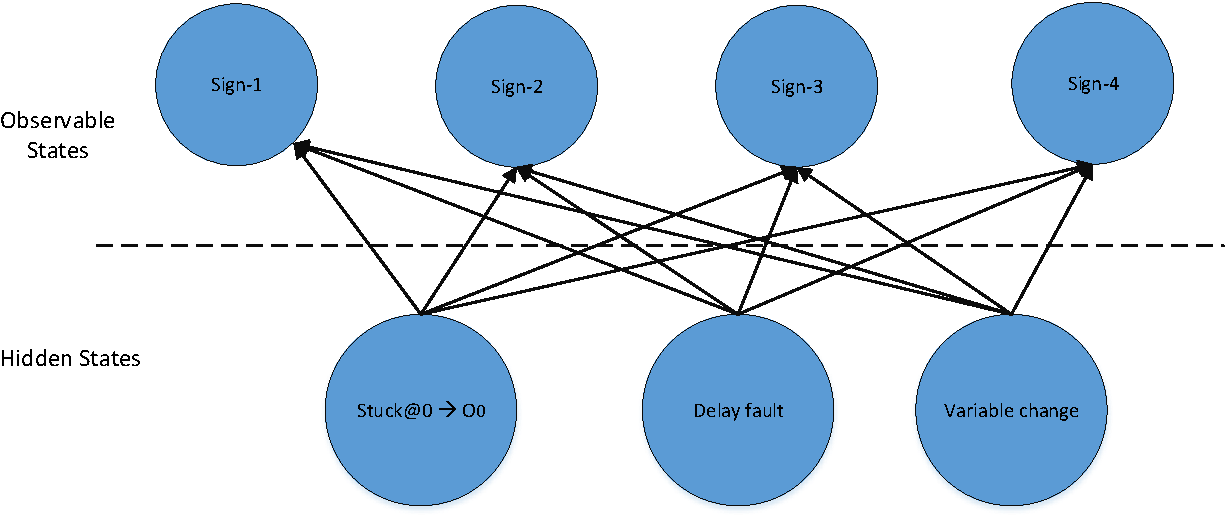
\includegraphics[scale=0.8]{Figures/HMM.pdf}
   \caption{HMM model 3-bit counter.}
\label{fig:ychart}
\end{figure}

\subsection{Probabilities in a HMM}

There are three important things to know about the probabilities in HMM

\begin{itemize}
\item The connections between the hidden states of the system, and the observable states of the system represent the probability of generating a particular observed state given that the Markov process is in a particular hidden state.

\item The probabilities entering into the observable states will sum to "1." 

\begin{center}
$Pr(Sign-1|Stuck) + Pr(Sign-1|Stuck) + Pr(Sign-1|Stuck)  = 1 $
\end{center}

\item In addition, probabilities define the Markov process, we have another matrix termed as "confusion matrix", which contains the probabilities of the observable states given a particular hidden state. The following matrix is the confusion matrix for the 3-bit counter example.


\begin{center}


CM = \bordermatrix{~& Sign-1 & Sign-2 & Sign-3 & Sign-3\cr
                  Stuck@1--> & 0.60 & 0.20 & 0.15&0.05 \cr
                  Stuck@1--> & 0.25 & 0.25 &0.25 &0.25\cr
                  Stuck@1--> & 0.05 & 0.10 &0.35 &0.50\cr}
\end{center}
\end{itemize}


\subsection{HMM Parameters}

A hidden Markov Model is described as $(\Pi, A, B)$, Where,


\begin{center}

$\Pi = (\pi_i)$ initial state probabilities vector;

$A = (a_ij)$ state transistion matrix;  \hspace{0.3cm} $P_r(x_i | {x_j}_{t-1})$

$B = (b_ij)$ confusion matrix;     \hspace{0.3cm}        $P_r(y_i | x_j)$



\end{center}  


Once a system can be modeled as a HMM, it helps to find three problems.

In general terminologies, the first two are pattern recognition problem. We model this according to our problem, i.e.,

\begin{tcolorbox}[width=\textwidth,colback={gray},title={Evaluation },colbacktitle=gray,coltitle=black]  

Find the probability of an observed signature given a HMM.  
\end{tcolorbox}


\begin{tcolorbox}[width=\textwidth,colback={gray},title={Decoding },colbacktitle=gray,coltitle=black]  

Finding the hidden states that most probably generated an observed sequence. 
\end{tcolorbox}

\begin{tcolorbox}[width=\textwidth,colback={gray},title={Learning },colbacktitle=gray,coltitle=black]  

The third problem is generating a HMM given a sequence of observations.
\end{tcolorbox}



\section{HMM Solutions}

Hidden Markov Model can give the answer of three major questions, compute the probability of a given sequence of observations, compute the most probable sequence of states, given a sequence of observations and learn the best model, given an observation.

In order to find the solution of these three questions:


\textbf{The Three basic HMM Problems and Solutions}

\begin{itemize}
\item Problem 1 : Probability Evaluation
 \begin{itemize}
 \item How do we efficiently compute the $P(O|\Pi)$ from the given observation sequence $O = {O_1, O_2,...,O_n}$.
 
  \begin{itemize}
  \item The possible solution is given by the Forward and Backward procedures.
  \end{itemize}
 \end{itemize}
\end{itemize}

\begin{itemize}
\item Problem 2 : Optimal State Sequence
 \begin{itemize}
 \item Given observation sequence $O = {O_1, O_2,....,}O_n$ and model $\Pi$ how do we choose a hidden state sequence $Q={q_1,q_2,q_3,...q_n}$
that is optimal, i.e., best explains the data. 
  \begin{itemize}
  \item The solution is provided by the Viterbi algorithm.
  \end{itemize}
 \end{itemize}
\end{itemize}



\begin{itemize}
\item Problem 3 : How do we adjust the paramters of the model $\Pi = {\pi, A, B}$ to maximize the likelihood $P(O|\pi)$ 
 \begin{itemize}
 \item Given observation sequence $O = {O_1, O_2,....,}O_n$ and model $\Pi$ how do we choose a hidden state sequence $Q={q_1,q_2,q_3,...q_n}$
that is optimal, i.e., best explains the data. 
  \begin{itemize}
  \item The solution is either Expectation-Maximization or Baum-Welch re-estimation.
  \end{itemize}
 \end{itemize}
\end{itemize}






\section{HMM Application for Signature}


\subsection{Evaluation Application}

For probability evaluation we need to compute the likelihood of an observation sequence $O = {O_1, O_2,...,o_t}$ given a particular HMM model $ \Pi = {A, B, \pi}$. The computation of this probability involves all the possible hidden state sequence and evaluate the corresponding probability. 

\begin{itemize}

\item  $P(O | \Pi) = \sum\limits_{\forall Q}^{} P (O | X, \Pi) P (X, \pi)$ 

\item For a specific state sequence $X = {x_1, x_2,...,x_t}, P(O | Q, \Pi):$

 \hspace {0.2cm} $P (O | X, \Pi) = \prod_{t=1}^{T} P (o_t | q_t, \Pi) = \prod_{t=1^{T} b_{x_t} (o_t)}$
 
 \item The probability of the state sequence $X$:
 \\
 \hspace {0.2cm} $ P (X | \Pi ) = \pi_{x_1} a_{x_1 x_2} a_{x_2 x_3},...,a_{x_{T-1} x_T}$
 
 \item The final expression we get:
 


$P (O | \Pi ) = \sum\limits_{x_1, x_2,..., x_T} \pi_{x_1} b_{x_1} (o_{x_1}) a_{x_1 x_2} b_{q_2} (o_{x_2}),..., a_{x_{T-1} x_T} b_{xT} (o_{xT})$

\item If there are $N^T$ possible state sequence, this approach becomes infeasible to apply or implement even for the smaller circuits.

\begin{itemize}
\item For N = 5 and T = 100, the order of magnitude --- $10^7$
\end{itemize}
 

\end{itemize}

This problem can be solved by using the Forward Algorithm:

\textbf{Example:} Consider an example where we have a number of HMM (a set of trplet $(\pi, A, B)$) describing different systems, and a sequence of observation, e.g., you will get these system by performing radiation/fault emulation experiments for hours and hours of testing. You have number of HMM in simulink library and want to know which HMM most probably generated the given sequence (signature).


We will use the forward algorithm to calculate the probability of an observation sequence given a particular hidden Markov Model, and find the most probable HMM. Suppose that you have a HMM that describe the stuck-at-node, and we also have a sequence of signatures. Suppose the stuck-at-nodes works in this order $(stuck-at-c_0)$, $(stuck-at-c_1)$, $(stuck-at-O_1)$, the signatures: Sign-1, Sign-2, Sign-3. There is some hidden relationship between stuck-at-node and the signatures, we can make a "Trellis" diagram as shown in Figure....


From trellis figure we conclude the following:

\begin{itemize}

\item Each column in the trellis represents the possible state of the stuck-at-node and each state in column is connected to the each state in the adjacent column.

\item The transition between the states --- state transitions has the probability provided by the "state transistion matrix."

\item Each column in the signature observations at that time: the probability of this signature observation given anyone of the above stuck-at-node state is provided by the confusion matrix. 

\item As mentioned above one of the possibility of calculating the probabilities of the observed states would be find each possible sequence of the hidden stuck-at-node states and sum all these probabilities. Just for this example, there would be $3^3 = 27$ possible sequences, its extremely complex to do this. So, we used the forward algorithm that can calculate the probabilities of observing a sequence recursively given a HMM.

\end{itemize}

\textbf{Forward algorithm Steps:}

We need to calculate the probability of observing a signature recursively given a HMM. 

\begin{enumerate}

\item The first step is the initialization step at t = 1 when there is no path to the state. The probability of being at state at t = 1 is actually the initial probability:
\begin{itemize}


 \item $P (state | t = 1) = \pi $
\item The initial probability at t = 1 is the probability multiplied by the associated observation probability.
$\alpha(j) = \pi(j) b_i (O_1)$
\end{itemize}

\item Second, we need to define a \textbf{partial probability} which is the probability of reaching an intermediate state in the trellis.

\begin{itemize}

\item For example, the T-long signature sequence: $(Y_k1, Y_k2,..., Y_kT)$, the partial probabilities $\alpha 's$. Figure shows the Trellis diagram. Calculate the probability of reaching an intermediate state in the trellis diagram as the sum of all possible paths to that state.

\item The partial probability of state $j$ at time $t$ is $t(j)$, to calculate the partial probability:

$\alpha_t(j) = P (observation | hidden state is j) \times P (all paths to state j at time t)$

\item The partial probabilities for the final observation hold the probability of reaching those states going through all the possible paths. The sum of these final partial probabilities is the sum of all possible paths. 

\hspace {4.5 cm}$\alpha_{t+1}(j) = b_jk_{t+1} \sum\limits^{n}_{i = 1} \alpha_t(i) a_{ij}$




\end{itemize}
\item This expression can be used to calculate the $\alpha$. We can find the probability of an observation given HMM. The probability of the sequence given the HMM is then the sum of the partial probabilities at time t = T. This is called termination step.
 
 \hspace {4.5 cm}$P(Y^K) = \sum\limits^{n}_{j=1} \alpha_T (j)$

\end{enumerate}







\subsection{Decoding Application}
The decoding capability of HMM helps to find the sequence of hidden states that generated the given observed output. In the FPGA fault emulation and radiation experiment we are interested to find the hidden states of the system as they represent some valuable information that can later used to give to the Simulink model.
 
\textbf{Example:} Consider an example of the signature and stuck-at-fault; an FPGA test designer can only sense the signature but wants to know the stuck-at-fault node, i.e., hidden state.
\textbf{Answer}: We will use the \underline{Viterbi Algorithm} to determine the most probable sequence of hidden states that give the sequence of observations and HMM. Inshort, decoding helps to find the hidden sequence most likely to have generated a sequence of observation --- solved using Viterbi algorithm.
\subsubsection{Viterbi Algorithm}


The Viterbi algorithm is based on the assumption that the most \textit{likely} path (hidden states sequence), $Q^* = argmax_Q P(Q|O) $, is a good estimation of the sequence of hidden states that generated the observed sequence $(O)$. The viterbi algorithm generates a path $X = (x_1, x_2,...,x_T)$, which is a sequence of states $x_n \in S = {s_1, s_2,...,s_k}$ that produce the sequence of observations $Y = (y_1,y_2,...,y_T) \in {1,2,...,N}^T N = Observation space$.

\textbf{Initialization:}



\begin{itemize}


\item The Observation space $O =  {o_1,o_2,...,o_N}$

\item the state space $S = {s_1,s_2,...,s_K}$

\item an array of the initial probabilities $\Pi = (\pi_1, \pi_2,...,\pi_K)$; $\pi_i is the probability the x_1 == s_i$

\item a sequence of observations $Y = (y_1,y_2,...,y_T)$; $yt == i$ the observation at time $t$ is $o_i$

\item the state transition matrix $A_ij$ stores the transition probability from state $s_i$ to $s_j$


\item emission matrix $B_ij$ stores the probability of observing $o_j$ from the state $s_i$
\end{itemize}  

\textbf{Recursion:}

We need to determine the hidden states by calculating $P(X|O)$. However, this brute force approach becomes intractable if the number of states gets larger, as the number of state path grows exponentially $(N^T)$. So, we need to calculate the $argmax_X P(X|O)$ . The most likely sequence is given by the recursion relations.

\begin{center}

\begin{itemize}


\item $V_1,k = P (y_1|k) \times \pi_k$

\item $V_t,k = max_{x \in S} (P (y_t|k) \times a_x,k \times V_t-1,x)$

\item $V_t,k$ probability of the most probably sequence $P (x_1, x_2,...,x_T, y_1,y_2,...,y_T)$

\end{itemize}

\end{center}


\textbf{Final:}

The most likely hidden state sequence $X = (x_1,x_2,...,x_N)$ 

\section{Case Study}


Consider you have an FPGA board, with some benchmark, e.g., counter is running on it. You need to  ask to perform a radiation induced experiment on it, drive the signatures, and make the high level model of it.

Suppose at any given time, the system can be in one of N possible states.

\begin{center}
$S = {S_1, S_2,....., S_N}$
\end{center}

From the experimental data you observed there are only three possible states in which system can go, e.g., stuck-at-1$\rightarrow O_{0}$, stuck-at-0$\rightarrow O_{1}$, and stuck-at-1$\rightarrow C_{1}$. I further observed that the transistion between these states can be described by the transition matrix.


\begin{center}


A = {$a_ij$} = \bordermatrix{~& & & \cr
                   & 0.4 & 0.3 & 0.3 \cr
                   & 0.2 & 0.6 &0.2 \cr
                   & 0.1 & 0.1 &0.8 \cr}
\end{center}

--- Question

\begin{itemize}
\item I model this behavior of the system in MATLAB and ask the high-level simulink designer you can find the response of the system as you like. He set the system paramters to know the faulty response of the system for the next seven different radiation experiment in order of (stuck-at-1$\rightarrow C_{1}$, stuck-at-1$\rightarrow C_{1}$, stuck-at-1$\rightarrow O_{0}$, stuck-at-1$\rightarrow O_{0}$, stuck-at-1$\rightarrow C_{1}$, stuck-at-0$\rightarrow O_{1}$, stuck-at-1$\rightarrow C_{1}$  ) given that the outcome of first radiation experiment is stuck-at-1$\rightarrow C_{1}$.

\item \textbf{Answer}


\item P(stuck-at-1$\rightarrow C_{1}$, stuck-at-1$\rightarrow C_{1}$, stuck-at-1$\rightarrow O_{0}$, stuck-at-1$\rightarrow O_{0}$, stuck-at-1$\rightarrow C_{1}$, stuck-at-0$\rightarrow O_{1}$, stuck-at-1$\rightarrow C_{1}$ | model)
\end{itemize}

\hspace{0.2cm} = P(stuck-at-1$\rightarrow C_{1}$) P(stuck-at-1$\rightarrow C_{1}$| stuck-at-1$\rightarrow C_{1}$) P(stuck-at-1$\rightarrow C_{1}$| stuck-at-1$\rightarrow C_{1}$) P(stuck-at-1$\rightarrow O_{0}$|stuck-at-1$\rightarrow C_{1}$) P(stuck-at-1$\rightarrow O_{0}$|stuck-at-1$\rightarrow O_{0}$) P(stuck-at-1$\rightarrow C_{1}$|stuck-at-1$\rightarrow O_{0}$) P(stuck-at-0$\rightarrow O_{1}$|stuck-at-1$\rightarrow C_{1}$) P(stuck-at-1$\rightarrow C_{1}$| stuck-at-0$\rightarrow O_{1}$)

\hspace{0.2cm} = $\pi_3$ $\times$ $a_33$ $\times$ $a_33$ $\times$ $a_13$ $\times$ $a_11$ $\times$ $a_31$ $\times$ $a_23$ $\times$ $a_32$

\hspace{0.2cm} = $1 \times 0.8 \times 0.8 \times 0.1 \times 0.4 \times 0.3 \times 0.1 \times 0.2$

The above mentioned model assumes that each state can be uniquely associated with an observable event. This model is too restrictive to be used for most of the realistic problems like ours, where we have no information of the underlying system only observe the outcome due to the result of change in hidden state.


\subsection{Learning}

We can also find the optimal solution for our model by using the learning application of the HMM. The learning application works on the model parameters and observations to find the model that fits the data. There are three different techniques to do: a) Maximum Likelihood Estimation, b) Viterbi Training, and c) Baum  Welch = Forward-Backward Algorithm. 

The Baum-Welch works in the following way:

\begin{enumerate}


\item Find the forward probabilities with the forward algorithm
\item Find the backward probabilities with the backward algorithm
\item Find the contribution of the current sequence to the transitions of the model.
\item Find the contribution of the current sequence to the emission probabilities of the model.
\item Find the new model parameters (starting probabilities, transition probabilities, and emission probabilities).
\item Find the new log likelihood of the model.
\item Stop when the change in the log likelihood is smaller than a given threshold or the maximum number of iterations is being passed.

\end{enumerate} 














\section{High Level Error Analysis}






In digital sequential circuit, a single event upset cause a  faulty repose of the underlying circuit. Consider this faulty response occur due to the a node in the circuit stuck-at-1, now this node response that is stuck-at-1 as shown in Figure~ can propagate to multiple outputs, and produce multiple erroneous output. The way this SEU interrupt at high-level of abstraction could typical manifest multiple correlated; "change in states of the design", and "change in signature values."

Inorder to model the fault occur at low level, the faulty response of the circuit to high level of abstraction, I propose to use the Hidden Markov Model.


HMM is based on  the two things:a) Observabale States, b) Hidden States. If we closely observe above mentioned problem, we realized that in this scenario --  signatures are my observable state, and the fault occur due to the bit-flip that cause some node in the circuit to stuck, stuck-at-1 $\rightarrow$ Cin is the hidden state.

In this thesis, we propose a method based on the Hidden Markov Model to evaluate the severity of the faulty behavior induced by the SEUs as a high level behavioral level. 


Befor going into the details:

\textbf{Hidden States:} The true states of the system that may be descrobed by a Markov Process, e.g., Stuck-at-1, some particular node.

\textbf{Observable State:} The state of the process, visible, e.g., Signature (difference between original output and faulty output).

\textbf{$\Pi Vector$:} contains the probability of the hidden model being in a particular hidden state at time t = 1.

\textbf{state transition matrix:}  holding the probability of a hidden state given the previous hidden state.

\textbf{confusion matrix:} containing the probability of observing a particular observable state given that the hidden model is in a particular hidden state. 


\section{Sequential Circuit Emulation}

%\subsection{Emulation Environment and Framework}
%\subsection{Sequential Circuit Fault Injection Mechanism}
%\subsection{Sequential Circuit Test Generation}


\section{Modeling Faults in Sequential Circuit}
\subsection{Soft-Error Modeling and Analysis in Sequential Circuit}


To analyze the faulty behavior of the sequential circuit by using Markov Chain theory is quite obvious choice. Markov chain analysis provide the steady state behavior of the sequential circuit. By using MC analysis we will able to find the number of clock cycles the sequential circuit produce the faulty output.

As mentioned in the section related work, single error rate can be categorized into three different categories a)  circuit level b) gate level and c) architectural level.  Our work is focused on the architectural level by emulating the fault at circuit level. 




Most of the real-time application of the electronic systems are sequential in nature, e.g., random access memories. A typical sequential circuit comprises of combinational logic and flip-flop as shown in Figure.   Inputs of the combinational logic, output of the combinational logic, and inputs and outputs of the flip-flop. There is a temporal correlations between the input signal and the state signal. The state signals are uniquely identified as the function of the input signal and the previous state signal. Due to this; sequential circuit error propagation from the error site, e.g., a bit flip in a flip-flop to the output can observe after several clock cycles. This temporal relationship force to use the more dynamic models than the models availble for the combinational circuits. The sequential circuits models can evolve with the time instances.

We will make our faulty model from the real-time radiation experiment. We will start our analysis by analysing the faulty values. Let us consider the example of the counter as shown in Figure 1 fault free and Figure 2 faulty where output is stuck at 1 .  


We will start our analysis by error probability matrix associated with the circuit and the probability that the erros comes in any part of the circuit (Combinational or flip-flop) produce an error at the output. 





\section{Markov Chain Analysis for Faulty Behaviour Model}

   
We used the MC for modeling and analysis of sequential circuits susceptible to soft-errors. We prefer to use Markov chain analysis over the other techniques like BDD/ADD or SAT, As these techniques requires to transform the circuit into their respective tool or mathmatical notation. While, in MC we can directly make the model just looking into the signature values. 


The faulty behaviour of a sequential circuit can be analyzed using MC theory. We need to calculate the steady state behaviour of a sequential circuit via MC analysis. 

Inorder to do the MC analysis. We need to have a two copies of the original circuit --- named Fault-Free circuit, and Faulty circuit (\textit{hit circuit}). The Fault free circuit is used to collect the correct behaviour of the circuit (fault-free outputs and fault free state vectors) and faulty is used to collect the faulty response of the circuit (faulty output and faulty states). From Markov theory, we can define the next state vectors of the fault-free and faulty circuit as:




$NS^{original}$ $=$  $\delta^{o}$ $=$ $(\delta^{o}_{1},\delta^{o}_{2},\delta^{o}_{3},...,\delta^{o}_{m})$


$NS^{faulty}$ $=$  $\delta^{f}$ $=$ $(\delta^{f}_{1},\delta^{f}_{2},\delta^{f}_{3},...,\delta^{f}_{m})$


$\delta^{o}$ $=$ Fault-Free circuit output values

$\delta^{f}$ $=$ Faulty circuit output values

$m$ $=$ Number of output variables

From there I can construct my signature vector:


$\epsilon_{signature}$ $=$ $\delta^{o}$  $-$ $\delta^{f}$


Now, the main goal for the soft error analysis for sequential circuits is to find the transistion probabilities between the signatures from the signature vector $\epsilon_{signature}$ and from there to determine the faulty behaviour of the sequential circuits when soft-error occurs. 

\subsection{SER Measurement in Sequential Circuits}

\subsection{Modeling with Probabilistic Calculation Methods}

%\subsection{Modeling of Sequential Circuit with Markovian-Chain Analysis}



%The fault injection platform proposes for this project emulates SEUs, more specifically single-bit upsets (SBUs) within the configuration memory of SRAM-based FPGAs. We will study the effects of SEU on sequential circuits, and introduce a  framework for analyzing and detecting them. We will do the modeling and analysis of sequential circuits susceptibility to soft errors. Accurate sequential SEU estimation requires capturing the mechanism of error propagation and masking at both combinational and sequential levels. The challenging task for the sequential circuits under SEUs: the difference between sequential and combinational circuits from the context of ATPG and single stuck-at fault model. In this project, we will concentrate on sequential synchronous circuits. The problem we will face and encounter that the controllability of auxiliary inputs and observability of secondary outputs for the sequential circuits.  We will study and implement a technique which eases sequential circuits testing and ATPG by making controllability and observability much simple.
%
%\subsection{Fault Injection}
%
%We need to examine the behavior of a design under faults. For fault injection there are two strategies: (a) \textit{Software based fault injection}, and (b) \textit{FPGA based fault injection}. 
%
%\begin{itemize}
%
%\item Two methods will develop for software based fault injection. First, the source HDL code is modified to allow fault injection. Second, the simulation tool is used to force the error injection during simulation. 
%\item For FPGA-based simulation, we will use single error mitigation core from Xilinx~\cite{xilinx}. The idea is to integrate this core with our system to generate a modified bitstreams to emulate the occurrence of errors. We will use this strategy.
%\end{itemize}





%\section{Research Axis 3: Radiation Bombardment}
This part of the project is a neutron-induced Single Event Effect test in a commercial FPGA from Xilinx. The primary objective is to investigate the radiation effects reliability for the critical application. We will implement the sequential circuit and data acquisition system. The results we want to achieve to drive signatures for the sequential circuits. Our focus is on the analyzing the impact of multiple errors in state flip-flops, during the cycles following the cycle when faults occur. The following milestones we want to achieve from radiation bombardment experiment.

\begin{itemize}
\item Modeling of SEU, MBU and analyzing their effect on logic circuits.
\item Evaluation of changes in error rates due to SEUs in sequential circuits.
\item Compute the error probability, and signatures from bit-upsets can vary for different outputs and different circuits. 
\item Evaluation of the impact of multiple flip-flop upsets in sequential circuits.
\item Determining the outputs that are most susceptible to errors due to faults in logic.
\item Determining the parts of the circuit (gates or gate clusters) that have the largest impact on circuit error probability.
\item Estimation of lower and upper bounds of circuit susceptibility to transient.
\end{itemize} 
%
%\section{Research Axis 3: High-level Modelling}
%
%To model and analyze the sequential circuit susceptibility to soft errors, we need to used the approximate methods, e.g.,
%\begin{itemize}
%
%\item Binary Decision Diagram and Algebraic decision diagram.
%\item Markov-chain analysis based error rate estimation, which can provide steady-state Single-Error rate estimates following a hit. 
%\item A  Monte Carlo for SEU Analysis of Sequential Circuits based on the probability of the bit-flips and estimates the states outputs and signatures.
%
%\end{itemize}
%\subsection{Simulator}
%
%We also have a plan to develop a simulator with the help of \textit{isoneo}. The simulator is based on the Matlab / Simulink models. The simulator takes the input a parameterization file corresponding to the operational architecture of the system. This file is generated from the configurator; it is in XML format.
%From this configuration, the simulator initially initializes a model of the system failure tree.
%This model is then exploited dynamically during the simulation phase to evaluate the level of reliability of the system and its components. The simulator executes the simulation model with the constraints and concludes a level of safety for each equipment and the global system.

\section{Optional: Fault Mitigation}
Fault-mitigation can be achieved in two ways: preventing faults from happening and
recovering after their occurrence. Fault preventing is achieved by using hardened components and/or shielding. But fault preventative is not a viable solution in terms of a project cost. More complex fault-mitigation methodologies can be implemented at the architectural level. We need to develop some fault-mitigation strategies like triple module redundancy with  dynamic reconfiguration of the hardware~\cite{jacobs2012reconfigurable} and/or something like the work presented in 
%Jacobs \emph{et al.}~\cite{jacobs2012reconfigurable} and Alderighi \emph{et al.}~\cite{violante} promote the use of SRAM-FPGAs for reconfigurable fault-tolerant space applications.
~\cite{jacobs2012reconfigurable} used fault tolerance framework (RFT) that enables system designers to dynamically adjust a system's level of redundancy and fault mitigation based on the varying radiation incurred at different orbital positions. Notably, the reconfigurable fault tolerance framework in~\cite{jacobs2012reconfigurable} is based on an upset rate modeling tool that used to capture time-varying radiation effects in a given orbit.


\section{Project Plan}


\textbf{Summary}

\textbf{Phase  01:} The emulation platform will be the starting point of research. We will use the SEUs for the configuration memory upsets. Selection of a suitable benchmark, which is probably ITC'99~\cite{ITC}used for the testing purpose. We will evaluate the bits sensitivity as well. We will implement the prototype. 

\textbf{Phase  02:} Evaluate the experimental setup under the neutron radiation at Triumf.


\textbf{Phase 03:} Develop an efficient methodology and high-level model for soft-error of sequential circuits, i.e., Monte-Carlo sampling, approximate approaches, symbolic methods for efficient estimation. The simulator development will keep with all these three phases.



%\section{Timetable}
%The development of the tasks identified in Chapter~\ref{sec:approach}, and the most important milestones of this project are presented in Figure~\ref{timetable}.
%In our intentions, the design of a time predictable computer architecture, the development of novel timing analysis techniques, and the FPGA prototypes implementation will unfold as a series of sequential tasks with relatively small interleaving. Dependability and real-time requirements, on the other hand, should be kept in mind throughout the whole advancement of the project.
%
%\begin{figure}[h]
%\centering
%\begin{tikzpicture}
%\begin{ganttchart}[
%x unit=0.36cm,
%y unit title=1.0cm,
%y unit chart=1.5cm,
%%vgrid,
%hgrid,
%inline,
%]{1}{48}
%\gantttitle{Research Project}{48} \\
%\gantttitle{2016}{12} \gantttitle{2017}{12} \gantttitle{2018}{12} \gantttitle{2019}{12}\\
%
%
%
%\ganttbar[bar height=.4]{Literature Review and Comp .Exam}{6}{24}\\
%%\ganttmilestone[]{Comp. Exam}{20}\\
%%\ganttmilestone[]{AHS}{6}
%%\ganttmilestone[]{TODAES}{12}\\
%\ganttbar[bar height=.4]{Emulation Platform for Seq. ckt}{6}{35} \\
%\ganttbar[bar height=.4]{Radiation Experiment}{13}{24} \\
%\ganttbar[bar height=.4]{Modelling and Simulator}{25}{42} \\
%%\ganttmilestone[]{TAAS}{30}\\
%%\ganttbar[bar height=.4]{Novel Timing analysis techniques}{22}{38} \\
%%\ganttmilestone[]{DAC}{36}\\
%%\ganttbar[bar height=.4]{FPGA Implementation}{27}{38} \\
%%\ganttmilestone[]{TRETS}{40}\\
%\ganttbar[bar height=.4]{Tech. Demo.}{35}{42} \\
%%\ganttmilestone[]{IAC}{44}\\
%\ganttbar[bar height=.4]{Thesis Writing}{35}{46}
%%\ganttmilestone[]{Thesis}{44}\\
%%\ganttbar[bar height=.4]{The \emph{PolyOrbite} Project}{1}{44} 
%
%%\ganttlink{elem0}{elem1}
%%\ganttlink{elem0}{elem2}
%%\ganttlink{elem0}{elem3}
%
%%\ganttlink{elem3}{elem4}
%
%%\ganttlink{elem5}{elem6}
%%\ganttlink{elem5}{elem7}
%
%%\ganttlink{elem7}{elem8}
%\end{ganttchart}
%\end{tikzpicture}
%\caption{Timetable.}
%\label{timetable}
%\end{figure}









